\documentclass[../main.tex]{subfiles} % required, if the Chapter be a seperate doc

\begin{document}

\section{Einleitung}\label{sec:einleitung}



    \subsection{Physikalischer Hintergrund}\label{subsec:physikalischer-hintergrund}
        Das \textbf{Federgesetz} – oder, auf mehrere Gegenstände übertragen, das \textbf{Hookesche Gesetz}\footnote{Gemeint ist Robert Hooke, der das Gesetz 1676 erstmals als Anagramm und 1678 aufgelöst publizierte} – beschreibt ein linear-elastisches Verhalten eines Materials, solange es sich innerhalb seiner elastischen Grenze befindet.

        Den Begriff \("\)Federgesetz\("\) verwenden wir hier als Oberbegriff für das Hookesche Gesetz in Bezug auf Federsysteme.
        Mit dem Hookeschen Gesetz modellieren wir einen linearen Sonderfall des sogenannten Elastizitätsgesetzes.

        \begin{tcolorbox}[title=Ausholung für das Elastizitätsgesetz]
            Das \textbf{Elastizitätsgesetz} beschreibt, wie sich ein elastisches Material unter Belastung verformt und wie dabei Spannung und Dehnung zusammenhängen.
            Im Vergleich zum Hookeschen Gesetz umfasst es jedoch auch nichtlineare oder zeitabhängige Reaktionen des Materials.
        \end{tcolorbox}

        Hier ist dieser lineare Sonderfall (Das Federgesetz) nochmals in einer Mathematischen Formel ausgedrückt:

        \begin{equation}
            F = D \cdot \Delta l
        \label{eq:federgesetz_formel}
        \end{equation}

        Wobei ${\Delta l}$ die Dehnung ist, die weiderum von der Kraft ${F}$ abhängig ist.
        Aus dieser Abhängigkeit bekommen wir nun die Federkonstante ${D}$, die wir durch ${\frac{F}{\Delta l} = D}$ errechnen können.

        Die Federkonstante dient jetzt als Proportionalitätsfaktor in der vorher aufgezeigten Formel~\ref{eq:federgesetz_formel} und beschreibt die Steifigkeit der Feder.


    \subsection{Aufgabenstellung}\label{subsec:aufgabenstellung}

        Die Arbeit stellt eine Zusammenarbeit der Fächer Physik und Mathematik dar.
        Ziel ist es, ein physikalisches Experiment zum Federgesetz durchzuführen, die Messdaten systematisch zu erfassen und anschliessend statistisch auszuwerten.
        Der Auftrag besteht darin, einen physikalischen Zusammenhang – das Federgesetz – zu untersuchen und die Ergebnisse mit Literaturwerten zu vergleichen.
        Zum schluss erfolgt eine Reflexion über unsere Resultate.
        Zusätzliche gibt es von den Teammitgliedern selbst noch jeweils eine Reflexion über die Arbeit.


    \subsection{Verwendete experimentelle Methoden}\label{subsec:verwendete-experimentelle-methoden}

        Experimente zum Federgesetz tragen im Internet viele Namen, jedoch kann man mit einer Feder nicht viel mehr Differenzen
        erzeugen wie einfach mit der Ausdehnung, wenn die Feder unter spannung steht und wann nicht.

        \subsubsection{Konzept}\label{subsubsec:konzept}

            \begin{figure}[h]
                \centering
                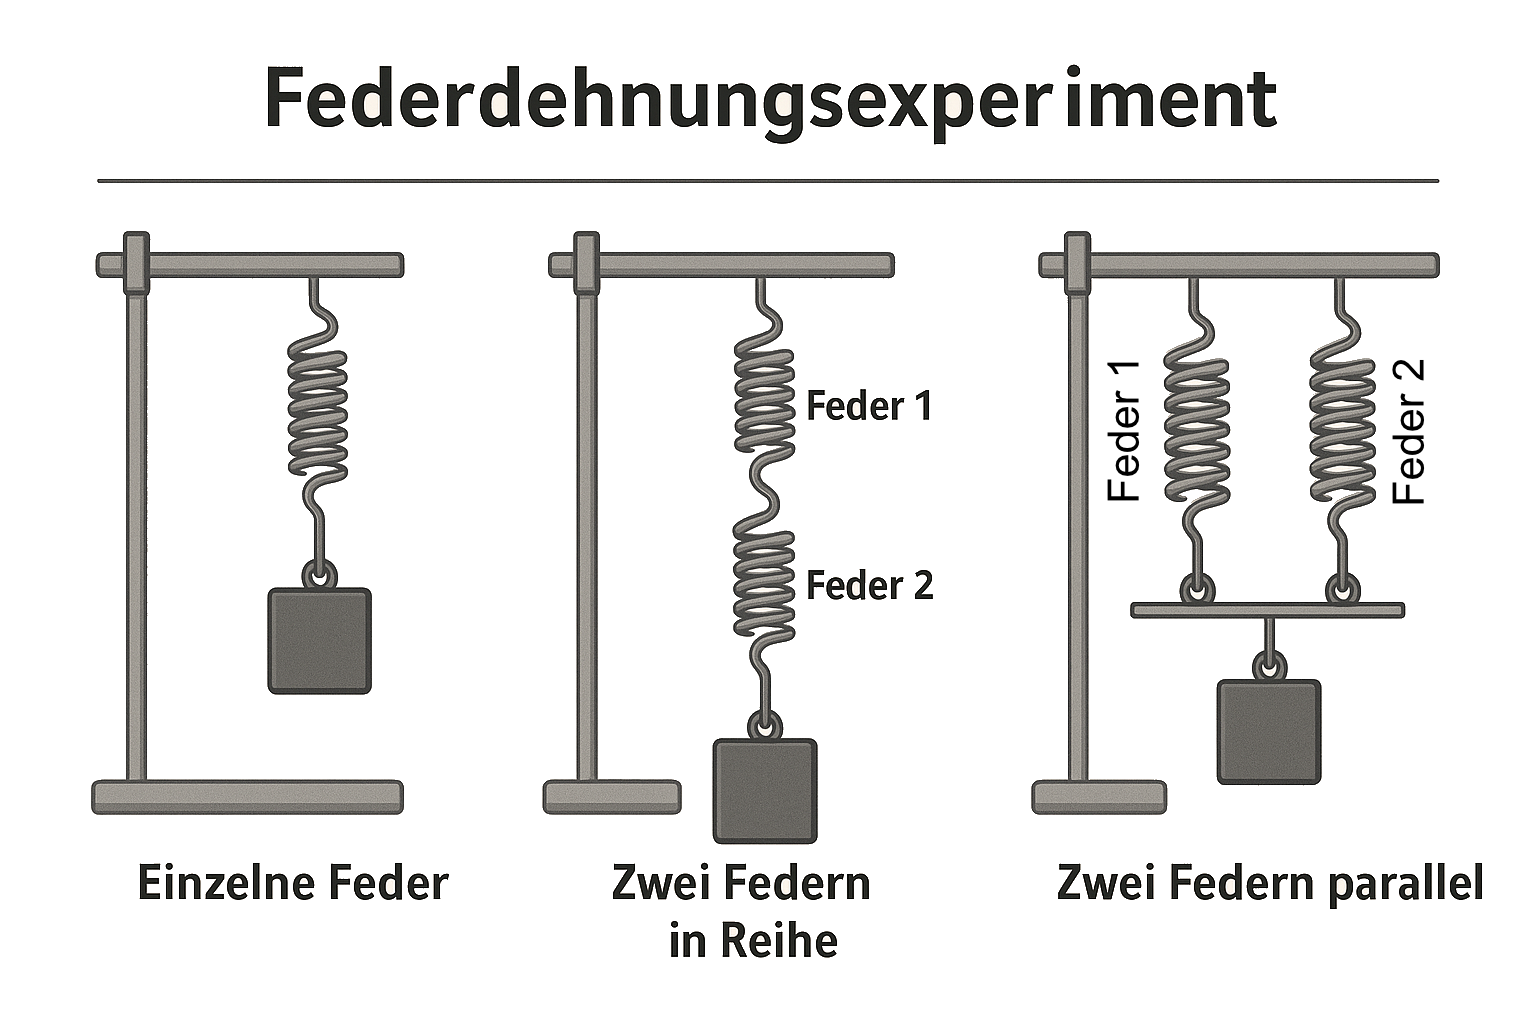
\includegraphics[width=0.7\textwidth]{Federdehnungsexperiment}
                \caption{Illustration zum Federdehungsexperiment. Zeigt einzelnen, seriellen und parallelen Teil des Federexperiments. KI generiert für Prompts sehe \ref{sec:generative-ki-nachrichtenverlaufe}}
                \label{fig:mesh1}
            \end{figure}

            Unser Experiment hat vier Phasen, siehe ~\ref{fig:mesh1} für bildliche Referenz.
            Die Phasen werden später (\ref{sec:experimenteller-teil}) genauer beschrieben, hier jedoch ein kurzer Überblick.
            \begin{enumerate}
                \item Beide Federn werden einzel mit den Gewichtsstufen bestückt und der Abstand zur gewichtslehren Position wird bestimmt.
                \item Auch beim zweiten und auch gleich beim dritten mal wieder die gleiche Übung hier sind die Federn jedoch nun Seriell angeordnet die Halterungen in der Mitte werden ignoriert.
                \item Kommen wir zu Phase drei: Nun sind die Feder parallel angeordnet und von einem Brett verbunden und mit Klammern an einem gemeinsamen gewicht befestigt und es wird wieder gemessen.
            \end{enumerate}

        \subsubsection{Material}\label{subsubsec:material}

            Um dieses Konzept nun in die Tat um zusetzten brauchen wir Folgendes:
            \textit{Die Nummern gehören zur Abbildung \ref{fig:material}}
            \begin{itemize}
                \item (7) Stativ-Stange
                \item (7) Stativ-Fuß
                \item (Abbildung \ref{fig:material3}) Muffe mit Klammer
                \item (6) Feder 1
                \item (6) Feder 2
                \item (4) Konstruktionslineal
                \item (5) Newton-Messgerät (Max. 1N)
                \item (5) Newton-Messgerät (Max. 6N)
                \item (1) Gewichthalterung mit Haken
                \item (3) 10x 10g Gewichte
                \item (2) 2x 50g Gewichte
                \item (Abbildung \ref{fig:material2}) Brett
                \item (Abbildung \ref{fig:material2}) 3x Klammern
            \end{itemize}
            \noindent
            Zusätzlich haben wir unsere Handys und Laptops für die Dokumentation genutzt.

            \begin{figure}[H]
                \centering
                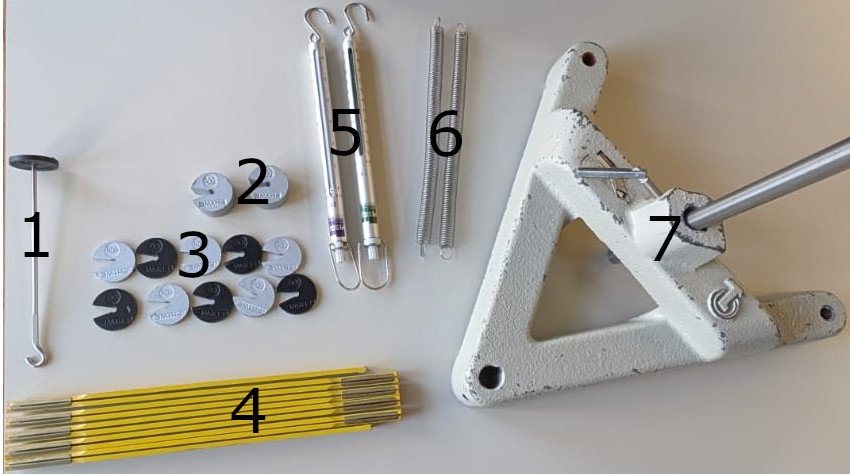
\includegraphics[width=0.6\textwidth]{materials/Materialien}
                \caption{Eigene Aufnahme des gebrauchten Materials siehe \ref{subsubsec:material}}
                \label{fig:material}
            \end{figure}

            \begin{figure}[H]
                \centering
                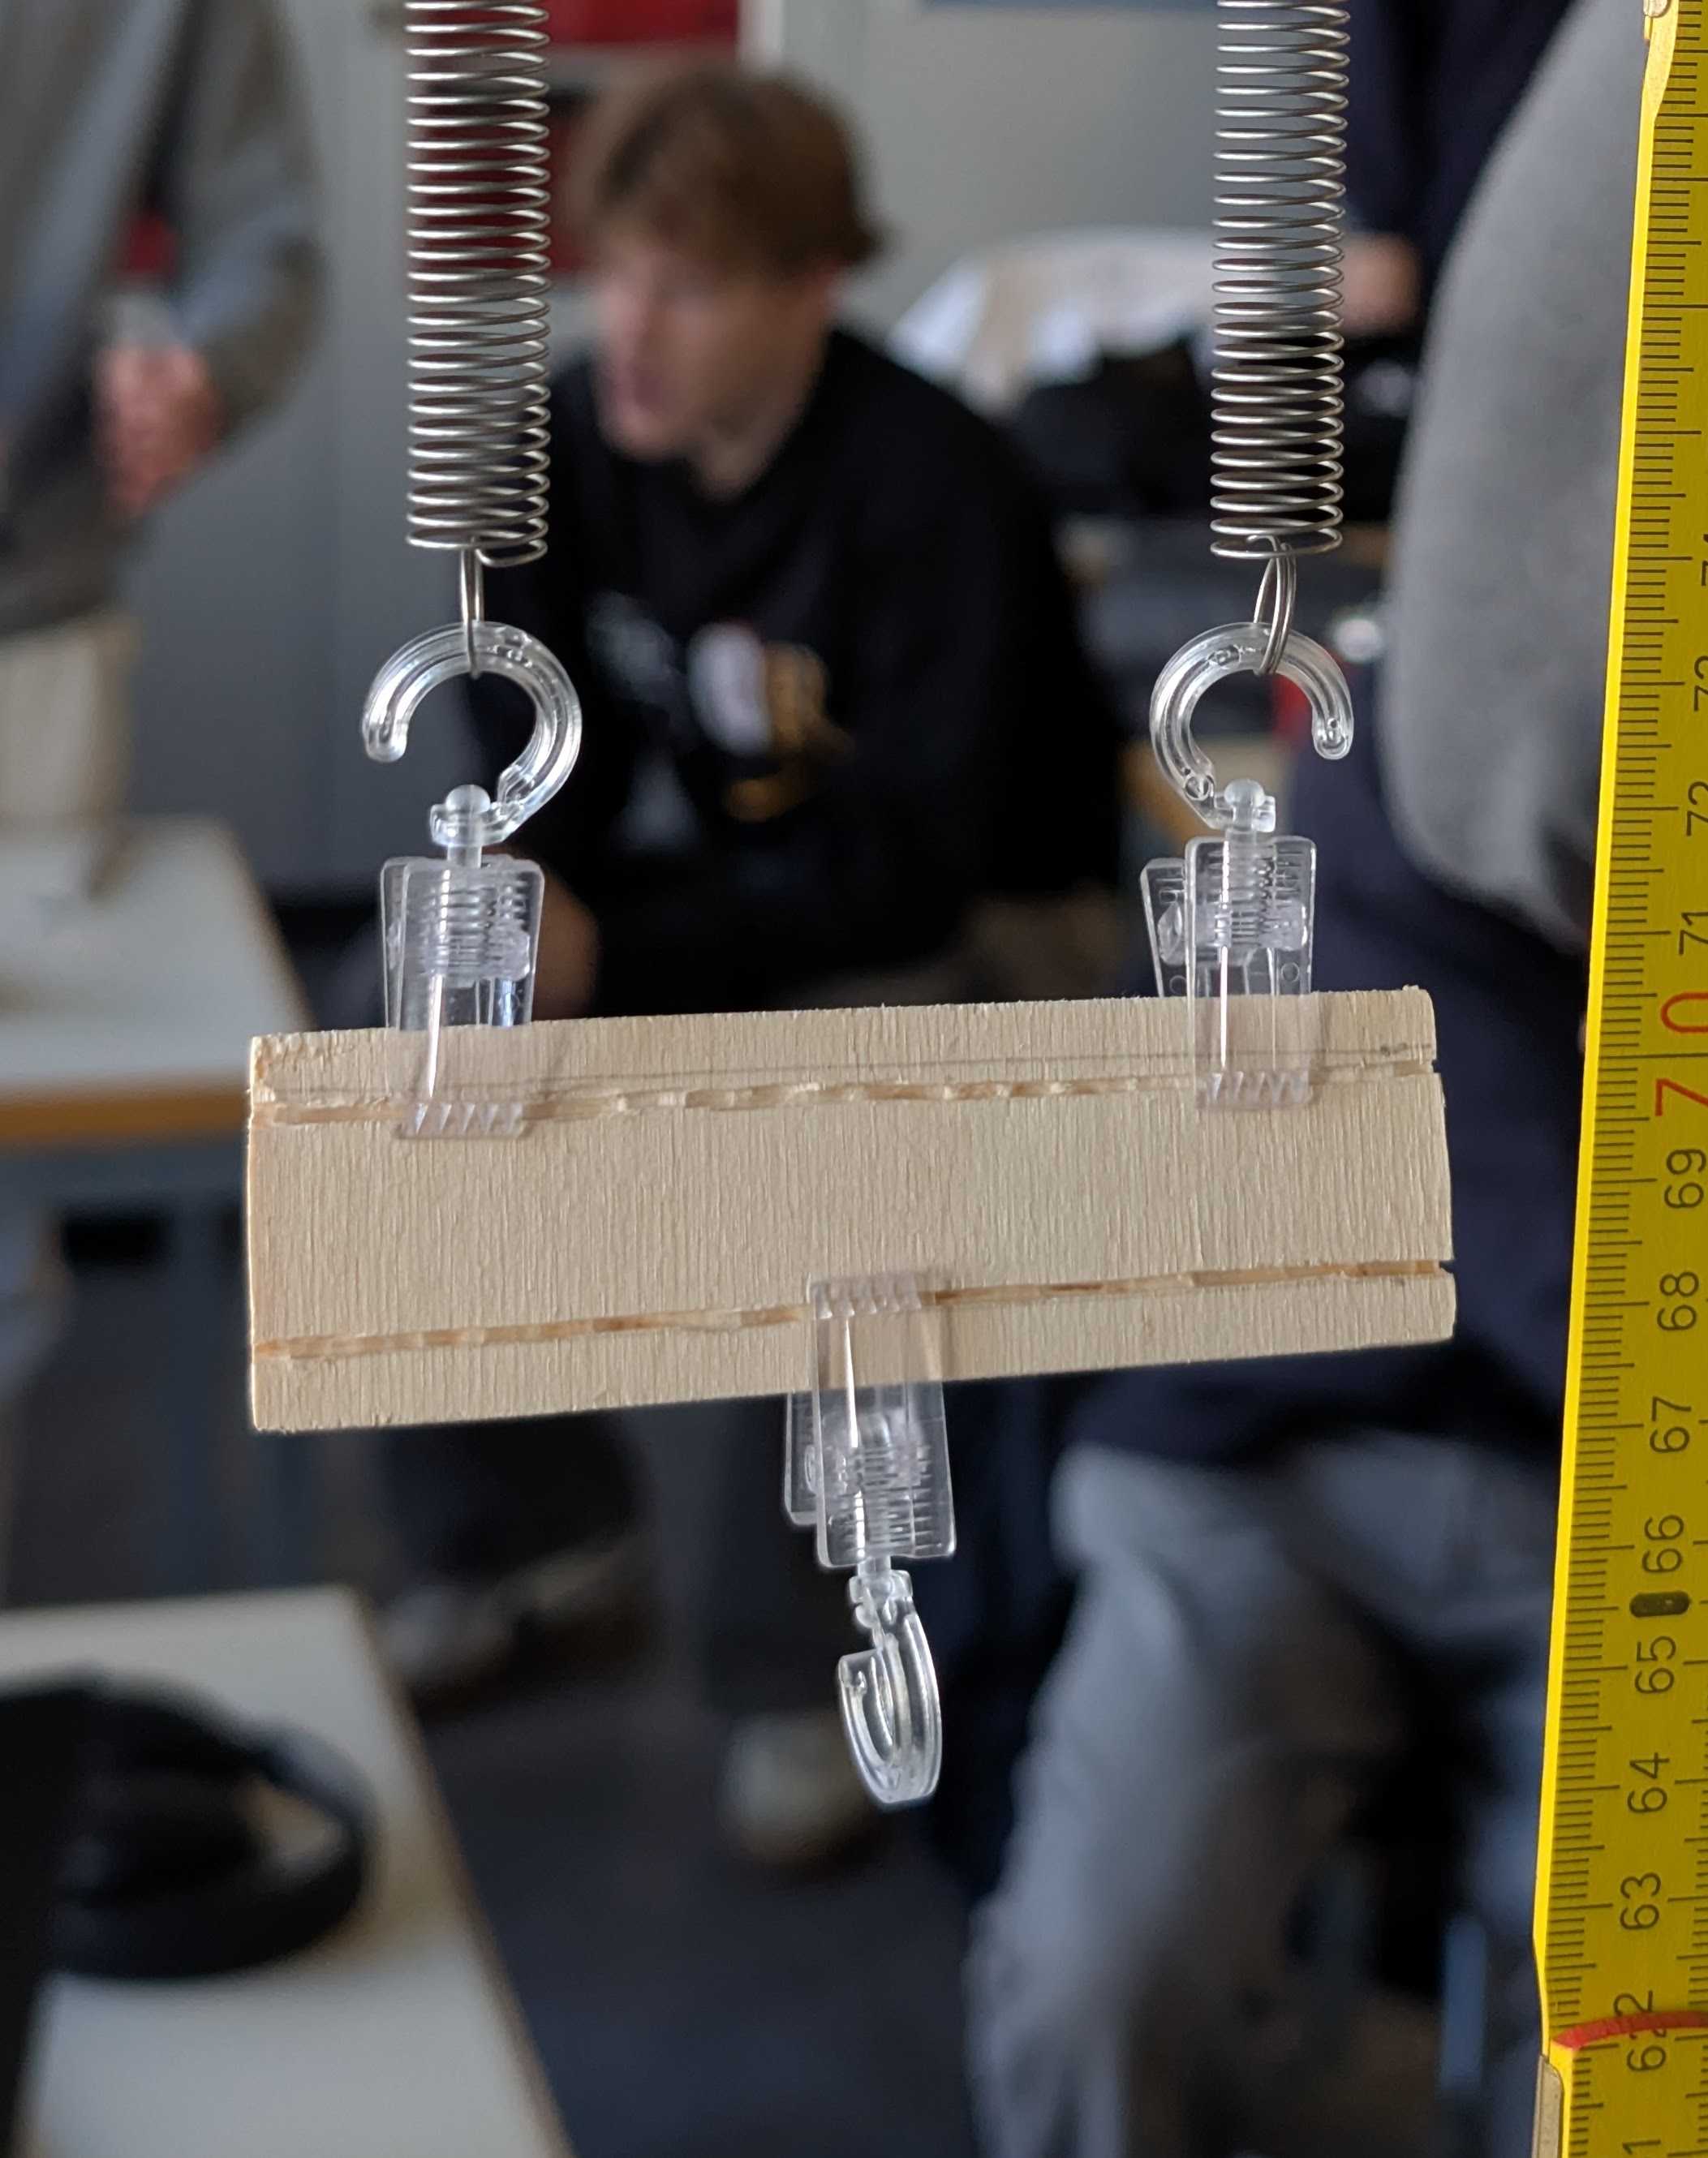
\includegraphics[width=0.4\textwidth]{materials/Materialien2}
                \caption{Eigene Aufnahme des Brettes und der Klammern im Einsatz \ref{subsubsec:material}}
                \label{fig:material2}
            \end{figure}

            \begin{figure}[H]
                \centering
                \includegraphics[width=0.3\textwidth]{materials/Materialien3}
                \caption{Eigene Aufnahme des obernen Teils der Experiment Vorrichtung  \ref{subsubsec:material}}
                \label{fig:material3}
            \end{figure}

    \subsection{Angewandte statistische Methoden}\label{subsec:angewandte-statistische-methoden}
        Um unsere Daten analyse und interpretieren zu können, haben wir die folgenden statistischen Methoden verwendet:
        \begin{itemize}
            \item $x$: \textbf{Arithmetischer Mittelwert} \\
            \quad Der klassische Durchschnitt – alle Werte addieren, durch die Anzahl teilen.
                  So können wir Zufallsfehlern entgegenwirken.

            \item $s$: \textbf{Standardabweichung des Einzel    wertes} \\
            \quad Ein Wert, der uns zeigt, wie weit unsere Zahlen streuen.
                  Desto höher dieser Wert desto mehr streuen die Werte.

            \item $\Delta \bar{x}$: \textbf{Standardabweichung des Mittelwertes (Standardfehler)} \\
            \quad Sagt dir, wie verlässlich dein Mittelwert ist.
                  Hier gilt auch desto kleiner desto verlässlicher und je höher die Zahl ist, desto mehr wurde gestreut unter den Mittelwerten.

            \item $R^2$: \textbf{Bestimmtheitsmass} \\
            \quad Misst den Erklärungsanteil der abhängigen Variable durch das Modell. $R^2 = 1$ bedeutet: Modell trifft ins Schwarze. $R^2 = 0$: reine Spekulation.
        \end{itemize}

\end{document}
